\documentclass[11pt,letterpaper]{article}
% Layout and typography for "One Photo Fewer".
\usepackage[T1]{fontenc}
\usepackage{iftex}
\ifPDFTeX\usepackage[utf8]{inputenc}\fi
\usepackage{amsmath}
\usepackage{newpxtext,newpxmath}
\usepackage{microtype}
\usepackage[letterpaper,top=1in,bottom=1in,left=1.15in,right=1.15in,headheight=14pt,headsep=20pt,footskip=30pt]{geometry}
\usepackage{booktabs,tabularx,array,graphicx,xcolor,enumitem,caption,fancyhdr,titlesec}
\usepackage{url}
\usepackage{flafter}
\definecolor{orisnavy}{HTML}{0D366B}
\usepackage[colorlinks=true,linkcolor=orisnavy,citecolor=orisnavy,urlcolor=orisnavy,pdfusetitle=false]{hyperref}
\setlength{\parindent}{1.3em}
\setlength{\parskip}{0pt plus 0.5pt}
\setlength{\emergencystretch}{1.5em}
\linespread{1.04}
\hyphenation{album albums}
\clubpenalty=9000 \widowpenalty=9500 \displaywidowpenalty=9500
\setlist{nosep,leftmargin=1.5em,topsep=4pt,itemsep=2.5pt}
% Headings
\titleformat{\section}{\normalfont\large\bfseries}{\thesection}{0.8em}{}
\titlespacing*{\section}{0pt}{16pt plus 3pt minus 2pt}{6pt plus 1pt}
% A bold run-in lead for a paragraph
\newcommand{\runin}[1]{\par\vspace{3pt plus 1pt}\noindent\textbf{#1}\enspace\ignorespaces}
% Header and footer
\pagestyle{fancy}\fancyhf{}
\fancyhead[L]{\small\textsc{One Photo Fewer}}
\fancyhead[R]{\small\textsc{Pantheon Labs}}
\fancyfoot[C]{\small\thepage}
\renewcommand{\headrulewidth}{0pt}
\fancypagestyle{firstpage}{\fancyhf{}\fancyfoot[C]{\small\thepage}\renewcommand{\headrulewidth}{0pt}}
% Captions and floats
\captionsetup{font=small,labelfont=bf,labelsep=period,skip=7pt,justification=justified,singlelinecheck=true}
\captionsetup[table]{position=top,skip=5pt}
\setlength{\textfloatsep}{14pt plus 3pt minus 2pt}
\setlength{\intextsep}{12pt plus 3pt minus 2pt}
\setlength{\floatsep}{12pt plus 3pt minus 2pt}
\renewcommand{\topfraction}{0.9}\renewcommand{\bottomfraction}{0.8}\renewcommand{\textfraction}{0.1}\renewcommand{\floatpagefraction}{0.75}
% A set-off quotation from the logs
\newcommand{\pull}[2]{\par\vspace{7pt plus 1pt}{\leftskip=1.6em\rightskip=1.6em\noindent\textit{#1}\par\vspace{1.5pt}\noindent{\small --- #2}\par}\vspace{7pt plus 1pt}\noindent\ignorespaces}
% Tables
\newcolumntype{Y}{>{\raggedright\arraybackslash}X}
\newcommand{\tablefont}{\small}
\renewcommand{\arraystretch}{1.12}

\hypersetup{pdftitle={One Photo Fewer: Inside the Oris Harness, Open-Weight Models Set 29 New Records for a Thirty-Year-Old Table of Mathematics},pdfauthor={Pantheon Labs},pdfsubject={Open-weight language models running inside the Oris research harness set 29 new covering-design records},pdfkeywords={Oris, research harness, open-weight models, covering designs, AI for mathematics, exact verification}}

\begin{document}
\thispagestyle{firstpage}

\begin{center}
\vspace*{2pt}
{\fontsize{23}{27}\selectfont One Photo Fewer\par}
\vspace{6pt}
{\large\itshape Inside the Oris harness, open-weight models set 29 new records\\[1pt] for a thirty-year-old table of mathematics\par}
\vspace{13pt}
{Pantheon Labs\par}
\vspace{1pt}
{\small AI Research Lab \textperiodcentered{} \href{mailto:contact@pantheon-labs.io}{contact@pantheon-labs.io}\par}
\vspace{5pt}
{\small November 2026\par}
\end{center}
\vspace{5pt}

\begin{center}\textbf{\small Abstract}\end{center}
\vspace{-5pt}
{\small\leftskip=2.2em\rightskip=2.2em\noindent
How few photos of nine can show every three of 41 guests together at least once? The best known answer was 168. In a single two-hour run inside Oris, the research harness built at Pantheon Labs, two open-weight language models found 167 and then broke two more public records, all within 28 minutes and with no person steering. GLM-5.3 wrote the search program, diagnosed and fixed its own bug from the program's log and chose where to aim it, while \mbox{DeepSeek-V4.1-Flash} scouted the literature. Across six runs in 47~hours, GLM-5.3 went from no record under an early version of Oris to 29 records in the next five runs, with \mbox{DeepSeek-V4.1-Flash} on the team: records in every run after the first, 16 in a single run and 216 photos saved in all. Every record comes with a certificate that a short script checks on a laptop, with no model and no Oris. The authors regard this as a breakthrough for open-weight models: inside Oris, they finished real mathematical work.\par}

\vspace{6pt}
{\small\noindent\textbf{Keywords}\enspace Oris; research harness; open-weight models; covering designs; AI for mathematics; exact verification\par}

\section{One photo fewer}

\noindent Forty-one guests. Every photo shows exactly nine of them. Every three guests must appear together in at least one photo. How few photos will do?

Nobody knows. The public table that records such things said 168, credited to Giovanni Acerbi in 2023 using lottery-wheel software, after 169 had stood for almost fifteen years. On 1~November 2026, seventeen minutes into a two-hour run that no person steered, a search job saved an album of 167 and printed \texttt{SOLVED}. A language model whose weights are public had written its program, and had repaired it less than three minutes earlier, after a number in its log stopped moving. Within eleven minutes, two more public records had fallen (Table~\ref{tab:records}).

The run took place inside Oris, the research harness built at Pantheon Labs. Forty-five hours earlier the same main model, then working alone under an early version of Oris, had found nothing. The web address of a public program built on the method that would win was on its screen inside two minutes, and that run never opened it. Over the next five runs, on five new versions of Oris and with a second open-weight model alongside, the models set 29 records.

This paper follows those six runs through their logs. Its thesis is that a model can know the recipe and still not finish, and that finishing can be engineered. It reports what went in, what came out and what each new version of Oris did differently. Every record can be checked without Oris.

\section{The puzzle}

Mathematicians call this a covering design and write the size of the smallest album as $C(v,k,t)$: $v$ guests, $k$ to a photo, every $t$ together \cite{gkp}. Each choice of the three numbers is one entry in a public table. Lottery players know the same puzzle as a wheel: 167 tickets of nine numbers guarantee that one ticket holds all three numbers drawn from 41.

One photo covers 84 of the 10,660 trios among 41 guests. Take 167 photos at random and about 2,844 trios are missed; about 1,173 photos are needed before the expected number missed falls below one, seven times the record. Yet checking an album takes a fraction of a second. Hard to find and easy to check: that is why this table suits machines, and why these results ask for no trust.

The table belongs to people. Dan Gordon started this one, the La Jolla Coverings Repository, in 1996, and its designs were, in his words, ``contributed by over a hundred people around the world over the past thirty years'' \cite{gordonpage}. He stopped taking submissions in March 2026 and archived a snapshot \cite{zenodo}. It continues as the Covering Repository, a lottery-wheel site run by Acerbi \cite{repository,gordonpage}. In 2026 it also became a proving ground for AI, with records from several AI-assisted efforts \cite{numaro,ozdemir,vanstaden}. Oris took it on with open-weight models only.

\begin{table}[!tb]
\caption{The three headline records, all from Run~6. ``Floor'' is the table's recorded lower bound. ``Kept'' counts photos unchanged from the public starting album. ``Minute'' is when the project's exact checking program, the referee, accepted the album; the 42-guest album delivered is a second one, accepted at 31.69, which shares no photo with the first. A \emph{record} here means below the lowest public value found on 3 November 2026.}\label{tab:records}
\tablefont
\setlength{\tabcolsep}{4pt}
\begin{tabularx}{\linewidth}{@{}rrrrYrrr@{}}
\toprule
Guests & Per photo & Trios & Floor & Old value, holder, date & New & Kept & Minute\\
\midrule
41 & 9 & 10,660 & 146 & 168, Giovanni Acerbi, Oct 2023 & \textbf{167} & 109 & 18.75\\
44 & 11 & 13,244 & 96 & 110, Alessandro Jurcovich, Apr 2022 & \textbf{109} & 70 & 27.86\\
42 & 12 & 11,480 & 63 & 75, WitnessFlow, Oct 2026 (table says 76) & \textbf{74} & 0 & 27.94\\
\bottomrule
\end{tabularx}
\end{table}

\section{The challenge}

Each run gave a team of model sessions a frozen rule book and a list of 2,095 entries (2,107 in the first run): 40 to 75 guests, up to 25 to a photo, every 3 to 5 together. The bar was the lowest value found: the table, public claims outside it, bounds implied by neighbouring entries and, from Run~3, the project's own earlier records. A tie did not count. The rule book barred copies, ``a design copied from anywhere else is not a result'', but not starting points, so the teams started from public albums. Every record was judged by the referee, the project's own exact program, kept separate from the models' work and read-only. Each run had two active hours on one shared 16-core machine, with the models running remotely.

Two open-weight models did the work: GLM-5.3, in all six runs, and \mbox{DeepSeek-V4.1-Flash}, from Run~2 \cite{glm,deepseek}. Oris is a general research harness, and Pantheon Labs built five new versions of it in the 45~hours between Run~1 and Run~6. The account below is drawn from the per-call logs of all six runs.

\section{The first try}

Two ideas run through this story. The \emph{removal idea}: start from a public album, delete a photo and repair the hole. The \emph{weighting idea}: make long-missed trios count for more.

Run~1 had both within reach. By minute~2 a session reading the literature had recommended repairing a public album downward, a GLM-5.3 session's reasoning held the removal idea, and a file it printed carried the address of Wynand van Staden's public repository \cite{vanstaden}, which holds a program built on the weighting idea. At least five sessions saw that address by minute~9. No session ever opened it.

At minute~26 a measure of what deleting one photo would leave missing, across 981 public albums, put two of Run~6's future winners at 6 and 9 trios short. The team picked other entries, and none moved. At minute~51 the weighting idea, tried on a toy puzzle in runs of under three seconds, was reported as ``REFUTED in a toy micro-test''. At minute~87 a session wrote ``the stall is the honest end state'', with 33 minutes left. Run~1 ended without a record.

The model knew the recipe. It did not finish. From Run~2 on, the team did: every later run set records (Table~\ref{tab:six}). One marker of the change is van Staden's page, never opened in Run~1 and asked for within 1.3 minutes in every later run, although the files those runs began with did not print its address. Figure~\ref{fig:clocks} sets Run~1 beside Run~6.

\begin{figure}[!tb]
\centering
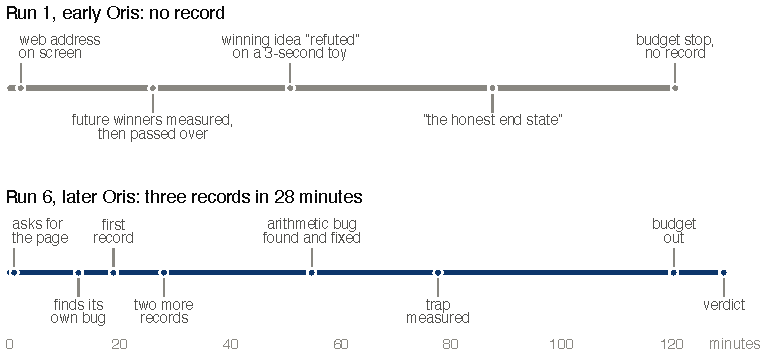
\includegraphics[width=0.93\linewidth]{figures/two_clocks.pdf}
\caption{Two runs on one clock: Run~1 under an early version of Oris, Run~6 under a later one, with \mbox{DeepSeek-V4.1-Flash} on the team.}\label{fig:clocks}
\end{figure}

\section{Twenty-eight minutes}

In Run~6 the two models split the work. GLM-5.3 made 1,373 of the run's 2,038 calls and wrote all the code, about 90 saved programs and 6,600 lines. \mbox{DeepSeek-V4.1-Flash} did 94\% of the web searches and page fetches; by minute~5.47 it had made 87 web searches, about as many as all of Run~1.

By minute~0.67, before its first file read, the recorded reasoning of a GLM-5.3 session held the removal idea. One minute in, a session reported that plain construction landed 47\% over the bar and asked whether a public album could be the start. Thirty seconds later a GLM-5.3 session answered: ``YES --- seeding is allowed'', on condition that the record be the team's own computation. The weighting idea reached the session writing the code near minute~6.9, from both models at once: Morris's ``breakout'' idea \cite{morris}, in a public program van Staden had just used to set records \cite{vanstaden}.

From minute~3 GLM-5.3 had been writing a search program in C, 273 lines by the end. It removes the weakest photo, picks a stubborn missing trio, finds a photo holding two of its guests and swaps in the third, keeps the swap if it helps and sometimes if it hurts, less often as the search goes on (it ``cools''), and when thousands of moves bring nothing, makes every missing trio count for one more. At minute~11.93 a test had found nothing, and a session wrote that a move counter was ``constant for 100s''. Half a minute later:

\pull{Now I understand the failure: moves/stag only count ACCEPTED moves, so once the annealer freezes (every move rejected at low T), stagnation never increments and breakouts stop firing --- dead search.}{a GLM-5.3 session, Run 6, minute~12.4}

In plain words, the counter ticked only on accepted moves, so once the search had cooled and rejected everything, the weighting step never fired. GLM-5.3 had written that bug five minutes earlier, and now it had traced it from the program's log. The fixed build came at minute~14.31. Another session, meanwhile, saw that its queue attacked the hardest entries first, killed its search and told the team: ``Rank your cells by closeness BEFORE burning core-hours.'' The three eventual record entries had ranked 288, 358 and 835 of 2,095 in the team's first ranking.

At minute~17.14 the first record appeared, 6 seconds into its search, and the referee accepted it at minute~18.75. The team kept going. The second record, 109 photos for 44 guests at 11 to a photo, took about 16 seconds of search and the third, 74 photos for 42 guests at 12 to a photo, about 426 (Table~\ref{tab:records}, Figure~\ref{fig:traces}). By minute~28 the referee had accepted all three. Those three searches total under 8 minutes, less than 1\% of the run's computing.

Two checks on running jobs each caught a real fault: a search that never searched, because its starting file did not exist, though the job would still have printed that it was done (``Your running-job check just paid for itself''), and swapped arguments that aimed results at a file named \texttt{150000000} (``that catch saved a false reproducibility story''). By minute~31.69 a variant of the program that cools by move count, not the clock, had produced a second 74-photo album, byte-for-byte reproducible, which shares no photo with the first and is the one delivered. GLM-5.3 wrote, aimed and fixed the program that found the albums.

\begin{figure}[!tb]
\centering
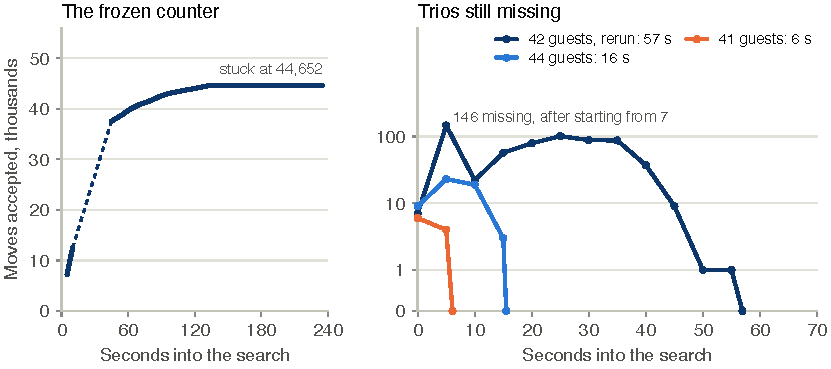
\includegraphics[width=0.93\linewidth]{figures/traces.pdf}
\caption{Left: the log that gave the bug away, on another entry before the fix (dashed across a gap between logged points). Right: the searches behind the delivered albums, with the time each took to reach zero. The 42-guest line is the rerun that produced the delivered album; it climbed to at least 146 missing before reaching zero at 57 seconds. The 426 seconds in the text belong to the first 74-photo album.}\label{fig:traces}
\end{figure}

\section{One seat short}

Close is not done. Remove the weakest photo from the public 41-guest album and only 6 of 10,660 trios go missing. But exactly one single-guest swap out of 48,096 helps, as a GLM-5.3 session measured during the run, and after it none does. Plain downhill stalls at once, so this search also accepts worse moves: in the rerun behind the delivered 42-guest album, 7 missing trios became 3, then 146 within five seconds, then none at 57 seconds on the full machine.

The most striking near miss was the 48-guest entry: 23 to a photo, 15 photos, where the table has said 16 since January 2009 and the floor is 15. A 600-second search reached 17,295 of 17,296 trios in five seconds and never improved. When a session's first theory collapsed, its next message said: ``My reading of the dynamics must be wrong somewhere.'' It logged the moves being rejected, found a true bug in one line of whole-number arithmetic and told the whole team at minute~55. The fix unfroze the search, and the search still stopped one trio short.

It was a trap, and a GLM-5.3 session measured most of it: at minute~77.6 it reported that its sampled stuck albums shared one form, with the three guests of the missing trio in 10 photos each, exactly two of them in every photo, and any swap that seats them breaking at least 108 other trios. A post-run analysis completed the picture. At least 7 of the run's 9 stuck albums (one kept, six rebuilt from the run's own programs) are one design with the names changed. Forty-five guests come in 15 sets of three who always appear together, plus 3 lone guests. Every photo holds 21 set members and 2 of the lone guests: exactly 23, exactly full. The one trio never photographed is the three lone guests. Seating them together needs seat 24 (Figure~\ref{fig:seat}). Appendix~\ref{app:math} proves what the trap is and leaves open whether 15 photos can ever be enough.

\begin{figure}[!tb]
\centering
\begin{minipage}[c]{0.33\linewidth}\centering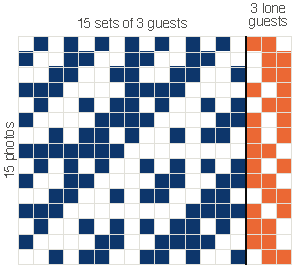
\includegraphics[width=\linewidth]{figures/one_seat_short.pdf}\end{minipage}\hfill
\begin{minipage}[c]{0.61\linewidth}
\caption{The stuck 48-guest album the run preserved. Every row is a photo with 7 dark squares (21 guests) and 2 orange (2 guests), so every photo is full at 23. No row has all three orange squares: that is the one missing trio.}\label{fig:seat}
\end{minipage}
\end{figure}

\section{Inside the albums}

A post-run analysis of the albums found hidden geometry in two of the three headline records. The 41 guests split as \mbox{25 + 16} and the nine seats as \mbox{5 + 4}: a 5-by-5 grid and a 4-by-4 grid. Exactly 100 photos pair a line of one grid with a line of the other. Those 100 are identical in the old record, the new record and a second 167-photo album made by rerunning the same command, and the two new albums share not one other photo (Figure~\ref{fig:inside}). The 44-guest album has the same kind of skeleton: \mbox{44 = 16 + 16 + 12} and \mbox{11 = 4 + 4 + 3}. The 42-guest album has a new pair of twins, two guests who now sit in exactly the same 21 photos. The program that lowered the records does not know what a line or a twin is. It kept the geometry it inherited and rebuilt most of what lay around it.

\begin{figure}[!tb]
\centering
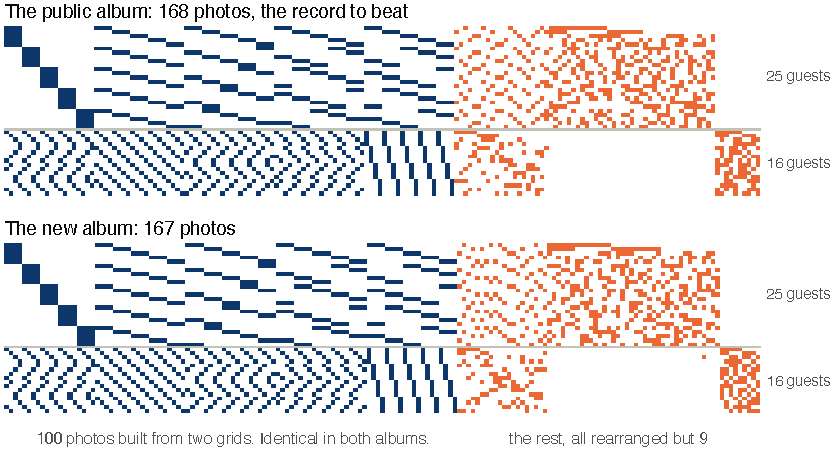
\includegraphics[width=0.74\linewidth]{figures/inside_record.pdf}
\caption{The old and new 41-guest albums, reordered by the geometry. Each column is a photo, each row a guest, and a mark means that guest is in that photo. The dark photos are the two-grid pattern, identical in both albums. The orange photos are where the search did its work.}\label{fig:inside}
\end{figure}

\section{Twenty-nine records}

After Run~1, every run set records: 4, 4, 2, 16 and 3 (Table~\ref{tab:six}). Nineteen of the 29 came from programs GLM-5.3 wrote, five from van Staden's public program, which the team found, aimed and launched, one from a published construction \cite{gkp} and four by deleting a guest from another record. Together they saved 216 photos against the bars; Table~\ref{tab:all} lists all 29. The largest single cut took $C(41,12,5)$ from 2,207 to 2,128, 79 photos fewer.

Run~5 was the best: 16 records, the first accepted at minute~6.40, on fewer web searches than any other run. One of its records started from Zarco's public 156-photo album \cite{zarco}: the team spotted a photo that covers nothing on its own and removed it, which alone beat the bar, and search then took the album to 143, within 5 of the floor of 138. Deleting guests from that album gave two more records.

\begin{table}[!tb]
\caption{Six runs side by side. Times are minutes. ``First record'' is its submission to the referee. ``Asked for page'' is the first request for van Staden's repository. ``Second model'' is \mbox{DeepSeek-V4.1-Flash}'s share of tokens.}\label{tab:six}
\tablefont
\begin{tabular*}{\linewidth}{@{\extracolsep{\fill}}lrrrrrr@{}}
\toprule
Run & Records & \shortstack[r]{Photos\\saved} & \shortstack[r]{First\\record} & \shortstack[r]{Asked\\for page} & \shortstack[r]{Web search\\calls} & \shortstack[r]{Second\\model}\\
\midrule
1 & 0 & 0 & none & never & 87 & none\\
2 & 4 & 10 & 28.08 & 0.46 & 363 & 5.0\%\\
3 & 4 & 4 & 12.40 & 1.30 & 110 & 1.5\%\\
4 & 2 & 2 & 54.22 & 0.70 & 655 & 9.9\%\\
5 & 16 & 197 & 6.36 & 0.83 & 86 & 0.9\%\\
6 & 3 & 3 & 18.67 & 0.75 & 376 & 6.1\%\\
\bottomrule
\end{tabular*}
\end{table}

\section{What changed with Oris}

Across the six runs the main model, the machine and the two-hour budget stayed fixed, and the bars never got easier: for 20 of the 29 record entries the bar was the same as in Run~1, and for the other 9 it was lower, so harder to beat. All eight records of Runs~2 and~3 rest on designs Run~1 already had. Around them the Oris setup moved fast: five new versions of the harness in 45~hours, \mbox{DeepSeek-V4.1-Flash} on the team from Run~2, longer source lists and changes to its web search service. The logs show what the new setup did differently.

\runin{Van Staden's page was opened at once.} In four of the five later runs, the first request for the page Run~1 never opened came from a \mbox{DeepSeek-V4.1-Flash} session, seconds after its own web search returned the address. In Run~5 named sources were fetched by minute~0.71 and the first record was accepted at 6.40. In Run~6 a source named in a note was followed up 17 seconds later, which led to the third record's starting album.

\runin{Faults were caught while the work ran.} Both Run~6 faults in Section~5 were caught by checks on jobs that were still running.

\runin{Results were banked faster, and jobs got more of the machine.} In Run~5 results waited up to 25 minutes before reaching the deliverables; in Run~6, 1 to 2 minutes. The median long job got 0.74 of the cores it asked for in Run~6, up from 0.40 in Run~2.

\runin{Run 6 ended on a verdict.} Run~1 stopped when its budget ran out, with no verdict. In Run~6 the budget ran out at minute~120.32 during the final check, and the verdict came 9 minutes later. That check rebuilt the program and regenerated the third record byte for byte in 21 seconds.

\section{What it means}

\runin{Inside Oris, open-weight models did real mathematical work.} They read the literature, built and debugged a program, aimed it, checked the running work and reported. No closed model took part in any run.

\runin{The thesis: finishing can be engineered.} Run~1 had the key pointer on its screen and the key idea in its reasoning, yet with 33 minutes still on the clock a session called the stall ``the honest end state''. The same main model, under later versions of Oris and with \mbox{DeepSeek-V4.1-Flash} on the team, set records in five runs straight. In the authors' reading, knowing lives in the model, and finishing is the harness's job.

\runin{A breakthrough for open-weight models.} The authors regard this as one. Two open-weight models, inside Oris, read a field; one wrote a program, diagnosed its own bug from the program's log, fixed it and aimed it, and across five runs the team left 29 records that anyone can check, each below the lowest public value in a table that people have been improving for thirty years. Oris is already at work on other problems.

\section{Verification}

The supplement is at \url{https://github.com/Ehsan187228/one-photo-fewer}. Its checks need Python 3.9 or later and nothing else: no network, no model, no Oris. \mbox{\texttt{python3 verify.py}} checks the three headline records in under a second, and \texttt{--all} checks all 29 in about a minute and a half. \texttt{check\_structure.py} rechecks the grids, the trap and both propositions in a few seconds. The 42-guest record also regenerates, with a C compiler, by rerunning GLM-5.3's search program from the supplement, in about half a minute.

The check does not ask which model found these albums or whom to trust. It counts trios.

\section*{Declarations}
{\small
\textbf{Competing interest.} Pantheon Labs develops Oris. \textbf{Models.} GLM-5.3 and \mbox{DeepSeek-V4.1-Flash} were the only models in the runs. \textbf{Oris.} Oris stays in-house at Pantheon Labs; its internals, prompts and raw logs are private. \textbf{Supplement.} All 29 certificates, the starting albums of the headline searches, data tables, check scripts and the two Run~6 search programs behind the headline records, written by GLM-5.3. \textbf{Credit.} The repository and its contributors \cite{repository,zenodo}, including Acerbi, Jurcovich, de Heer and Muir; van Staden \cite{vanstaden}; WitnessFlow (car-b) \cite{witnessflow}; Zarco \cite{zarco}; \"Ozdemir \cite{ozdemir}; the V3R1T4S contributors \cite{veritas}; mizopl \cite{clss}; Nurmela and \"Osterg\aa rd \cite{nurmela}; Morris \cite{morris}. La Jolla starting designs are used under CC BY 4.0, and the changes made are the searches described here.\par
}

\appendix
\section{For specialists}\label{app:math}
{\small
The structure below comes from post-run analysis of the albums. \texttt{check\_structure.py} rechecks the grids, the shared 100, the 64, the swap counts, the twins, the trap and both propositions. Coordinates are in the supplement.

\textbf{(41,9,3).} The points split as $A \cup B$, read as AG(2,5) and AG(2,4). Five of the six parallel classes of $A$ are matched with the five classes of $B$, and all 20 line pairs in each matched pair are blocks, giving the 100 core blocks. Two points of $B$ and one of $A$ always share a core block; two points of $A$ and one of $B$ do too, unless the pair lies on a sixth-class line. Lines of the sixth class of $A$ take 4-sets partitioning $B$ (20 blocks in the public design; in the record 19, and on the fifth line the last four points of $B$ sit three in a block of shape 6+3 and one in the block of shape 8+1). Each design has one block of shape 8+1 and 37 blocks inside $A$; blocks inside $B$ fell from 10 to 9.

\textbf{(44,11,3).} Points split as $P_1 \cup P_2 \cup Q$ with sizes 16, 16, 12 and labels in $\mathbb{Z}_2^4$, under which lines are cosets of the five subgroups of a spread and $Q$ is a third copy of the plane with one coset deleted. For each of the four other directions, a line of $P_1$, a line of $P_2$ and the coset completing their sum, which has lost exactly one point, form a block: 64 core blocks of size $4+4+3$, identical in the public design and the record.

\textbf{(42,12,3).} The public design has the twin pair $\{40,42\}$; the record keeps it and gains $\{15,31\}$.

\textbf{Proposition 1.} \emph{Let the 15 blocks be the points of PG(3,2). For each of the 15 planes add three design points lying in exactly the blocks of that plane. Partition the blocks into three ovoids $O_1,O_2,O_3$ (cosets of the order-5 subgroup of $\mathbb{F}_{16}^*$) and add points $x_i$ lying in every block outside $O_i$. Then $v=48$, $b=15$, $k=23$, and exactly one triple is uncovered.} Proof: each block lies on 7 planes and in exactly one coset, so it holds $21+2=23$ points. Three planes share a point. Two planes meet in a line, which no coset contains, so two planes and an $x_i$ share a point. A plane meets every coset, because the five points of a coset sum to zero and a plane therefore holds an odd number of them, so a plane, $x_i$ and $x_j$ share a point of $O_k$. The cosets cover all blocks, so $x_1,x_2,x_3$ share nothing. $\square$ The state preserved from Run~6 is this object. In dual terms its 45 plane points are a weighted blow-up of PG(3,2) with every weight 3, the construction used in Zarco's upper bounds \cite{zarco}. The $x_i$ are not points of that geometry: each lies in 10 blocks rather than 7, and a pure blow-up misses no triple.

\textbf{Proposition 2.} \emph{No 15 blocks of size at most 23 hold 48 points whose block sets are all planes of PG(3,2).} Proof: let $w(\pi)$ count points attached to plane $\pi$ and $e_p \ge 0$ the free seats in block $p$, so $\sum e_p = 15 \cdot 23 - 48 \cdot 7 = 9$. Summing over a plane's 7 blocks gives $161 - e(\pi) = 7w(\pi) + 3(48 - w(\pi))$, so $e(\pi) = 17 - 4w(\pi) \equiv 1 \pmod 4$ and the free seats off $\pi$ number 0, 4 or 8. These 15 numbers sum to $9 \cdot 8 = 72 > 60$, so some plane $H$ has 8 off and a single free seat $p$ on it. Take a plane $H'$ missing $p$, and $H''$ the third plane through $H \cap H'$. If $X$ of the other 8 seats lie on $H''$ but not $H'$, then $H'$ has $X+1$ off and $H''$ has $9-X$ off, which cannot both be multiples of 4. $\square$ This excludes no other shape, not even the trap's, whose $x_i$ lie in 10 blocks each, so $C(48,23,3)$ stays open between 15 and 16.

\textbf{Open questions.} Is $C(48,23,3)$ 15 or 16? All but one of the blocks of the 44-guest record fall into regular classes, and that block alone covers 12 triples, so could a 108-block $(44,11,3)$ exist? With the grids frozen, $(41,9,3)$ at 166 blocks leaves 3,330 triples for 66 blocks: could an exact method settle whether 66 blocks can cover them? Corrections, and the history of these constructions, are welcome at \href{mailto:contact@pantheon-labs.io}{contact@pantheon-labs.io}.\par
}

\section{All 29 records}\label{app:records}
{\small
All are valid under a fresh exact checker and under the referee of their run. Four follow from another record by deleting a guest, marked $\dagger$. In all, 216 photos were saved against the bars. Run~2 also produced six valid designs it did not deliver, among them $C(40,13,5)\le 1{,}329$, $C(72,14,5)\le 20{,}339$ and $C(73,14,5)\le 22{,}465$; they are not counted among the 29, and \texttt{verify.py --others} checks them.\par
}

\par\vspace{4pt}
\noindent\begin{minipage}{\linewidth}
\centering
\captionof{table}{Every record, with its new size and the bar it beat.}\label{tab:all}
\footnotesize
\renewcommand{\arraystretch}{1.0}
\setlength{\tabcolsep}{3.5pt}
\begin{tabular}{@{}lrr@{\hspace{1.5em}}lrr@{\hspace{1.5em}}lrr@{}}
\toprule
Run & Entry & New / bar & Run & Entry & New / bar & Run & Entry & New / bar\\
\midrule
2 & $C(40,13,5)$ & 1,332 / 1,338 & 5 & $C(41,12,5)$ & 2,128 / 2,207 & 5 & $C(69,24,4)$ & 119 / 121\\
2 & $C(53,21,5)$ & 386 / 387 & 5 & $C(61,20,5)$ & 1,168 / 1,169 & 5 & $C(71,25,4)$ & 120 / 124\\
2 & $C(72,14,5)$ & 20,341 / 20,342 & 5 & $C(62,14,3)^\dagger$ & 143 / 148 & 5 & $C(72,15,5)$ & 13,944 / 13,945\\
2 & $C(73,12,5)$ & 53,625 / 53,627 & 5 & $C(63,14,3)^\dagger$ & 143 / 156 & 5 & $C(72,25,4)$ & 123 / 124\\
3 & $C(41,18,4)$ & 68 / 69 & 5 & $C(63,14,5)$ & 10,111 / 10,114 & 5 & $C(74,16,3)^\dagger$ & 148 / 154\\
3 & $C(42,19,4)$ & 59 / 60 & 5 & $C(64,14,3)$ & 143 / 156 & 5 & $C(75,16,3)$ & 148 / 156\\
3 & $C(47,17,5)$ & 671 / 672 & 5 & $C(65,23,4)$ & 119 / 121 & 6 & $C(41,9,3)$ & 167 / 168\\
3 & $C(47,18,3)$ & 33 / 34 & 5 & $C(67,13,5)$ & 22,206 / 22,207 & 6 & $C(42,12,3)$ & 74 / 75\\
4 & $C(47,8,4)$ & 3,984 / 3,985 & 5 & $C(68,14,5)$ & 15,619 / 15,675 & 6 & $C(44,11,3)$ & 109 / 110\\
4 & $C(71,14,4)$ & 1,999 / 2,000 & 5 & $C(68,24,4)^\dagger$ & 119 / 121 & & &\\
\bottomrule
\end{tabular}
\end{minipage}
\vspace{2pt}

\par\ifdim\dimexpr\pagegoal-\pagetotal\relax<8\baselineskip\clearpage\fi
\begingroup
\footnotesize
\raggedright
\begin{thebibliography}{99}
\setlength{\itemsep}{0pt}
\item[] Web sources were read on 3 November 2026.
\bibitem{repository} The Covering Repository. \url{https://coveringrepository.com/}.
\bibitem{deepseek} DeepSeek-AI. DeepSeek-V4.1-Flash model card, revision 314113f. \url{https://huggingface.co/deepseek-ai/DeepSeek-V4.1-Flash}.
\bibitem{gkp} D.\,M. Gordon, G. Kuperberg and O. Patashnik. New constructions for covering designs. \emph{J. Combin. Designs} 3(4), 269--284, 1995. doi:10.1002/jcd.3180030404.
\bibitem{gordonpage} D. Gordon. Covering designs. \url{https://dmgordon.org/covering-designs/}.
\bibitem{zenodo} D. Gordon. La Jolla Coverings Repository, version 1.2. Zenodo, 24 Apr 2026. doi:10.5281/zenodo.19735294.
\bibitem{clss} mizopl. Compositional Lifting and Seam Surgery (CLSS). Zenodo, 2026. doi:10.5281/zenodo.23466237.
\bibitem{morris} P. Morris. The breakout method for escaping from local minima. \emph{Proc. AAAI-93}, 40--45, 1993.
\bibitem{numaro} Numaro AI Autoresearch Team. Covering-design records improving the La Jolla Covering Repository. NUMARO-2026-006, 2026. \url{https://numaro.tech/research/covering-designs-la-jolla-2026/}.
\bibitem{nurmela} K.\,J. Nurmela and P.\,R.\,J. \"Osterg\aa rd. Upper bounds for covering designs by simulated annealing. \emph{Congressus Numerantium} 96, 93--111, 1993.
\bibitem{ozdemir} K. \"Ozdemir. New upper bounds for 37 covering numbers $C(v,k,t)$. Zenodo, 2026. doi:10.5281/zenodo.23686233.
\bibitem{veritas} V3R1T4S contributors. Pull requests 211 and 398. \url{https://github.com/elder-plinius/V3R1T4S}.
\bibitem{vanstaden} W. van Staden. Local search and a construction scan for covering-design and lottery-covering tables. Preprints.org, 29 Oct 2026. doi:10.20944/preprints202610.2905.v1. \url{https://github.com/WynandVStaden/covering-design-records}.
\bibitem{witnessflow} car-b. WitnessFlow: code, protocols, results and covering certificates. Public research release, 2026. \url{https://github.com/car-b/witnessflow}.
\bibitem{zarco} A. Zarco. Covering numbers. \url{https://github.com/alejandrozarco/covering-numbers}.
\bibitem{glm} Z.ai. GLM-5.3 model card, revision ba32f8c. \url{https://huggingface.co/zai-org/GLM-5.3}.
\end{thebibliography}
\endgroup

\end{document}
